% File: co_po_pso_mapping.tex
% Place this file in the same folder as your main .tex, then use:
% \clearpage
% \addcontentsline{toc}{chapter}{Appendix C: CO--PO--PSO Mapping}
% \chapter*{Appendix C: CO--PO--PSO Mapping}
% % File: co_po_pso_mapping.tex
% Place this file in the same folder as your main .tex, then use:
% \clearpage
% \addcontentsline{toc}{chapter}{Appendix C: CO--PO--PSO Mapping}
% \chapter*{Appendix C: CO--PO--PSO Mapping}
% % File: co_po_pso_mapping.tex
% Place this file in the same folder as your main .tex, then use:
% \clearpage
% \addcontentsline{toc}{chapter}{Appendix C: CO--PO--PSO Mapping}
% \chapter*{Appendix C: CO--PO--PSO Mapping}
% % File: co_po_pso_mapping.tex
% Place this file in the same folder as your main .tex, then use:
% \clearpage
% \addcontentsline{toc}{chapter}{Appendix C: CO--PO--PSO Mapping}
% \chapter*{Appendix C: CO--PO--PSO Mapping}
% \input{co_po_pso_mapping}

\clearpage
	\addcontentsline{toc}{chapter}{Appendix C: CO--PO--PSO Mapping}
	\chapter*{}
	\paragraph\ 
	\vspace{75mm}
	\begin{center}
		\textbf{\huge{Appendix C: }}
		\textbf{\huge{CO--PO--PSO Mapping}}
	\end{center}
	% 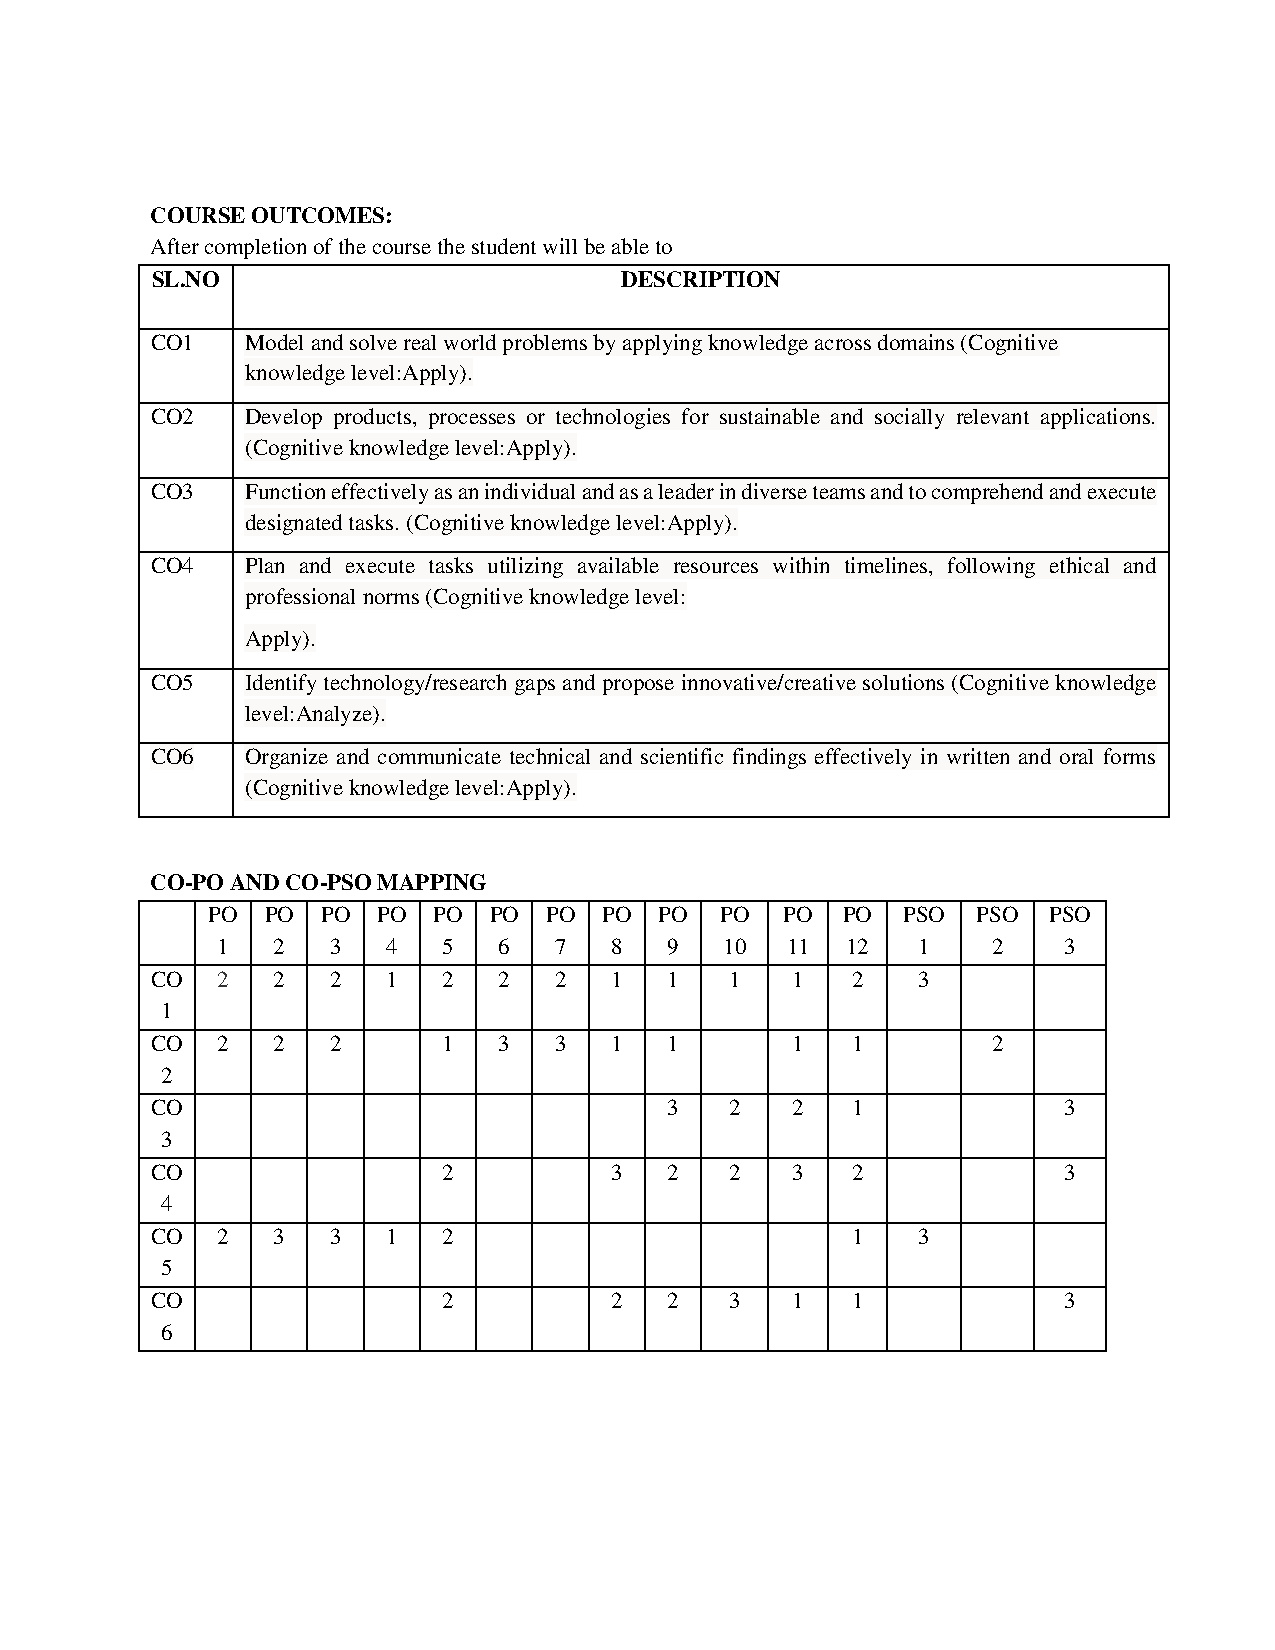
\includepdf[pages=-]{CO & jUSTIFICATIONS.pdf}
	
	\clearpage

\clearpage

% \addcontentsline{toc}{chapter}{Appendix D: CO-PO-PSO Mapping}
% \chapter*{}
% \paragraph\
% \vspace{75mm}
% \begin{center}
%     \textbf{\huge{Appendix D: }}
%     \textbf{\huge{CO-PO-PSO Mapping}}
% \end{center}
% \clearpage
% \clearpage





\vspace{1cm}

\begin{table}[htp]
\centering
\caption*{CO-PO AND CO-PSO MAPPING}
\scalebox{0.75}{
\begin{tabular}{|p{0.8cm}|p{0.8cm}|p{0.8cm}|p{0.8cm}|p{0.8cm}|p{0.8cm}|p{0.8cm}|p{0.8cm}|p{0.8cm}|p{0.8cm}|p{0.8cm}|p{0.8cm}|p{0.8cm}|p{0.8cm}|p{0.8cm}|p{0.8cm}|}
\hline
\textbf{} & \textbf{PO
1} & \textbf{PO
2} & \textbf{PO
3} & \textbf{PO
4} & \textbf{PO
5} & \textbf{PO
6} & \textbf{PO
7} & \textbf{PO
8} & \textbf{PO
9} & \textbf{PO
10} & \textbf{PO
11} & \textbf{PO
12} & \textbf{PSO
1} & \textbf{PSO
2} & \textbf{PSO
3} \\
\hline
\textbf{CO
1} & 2 & 2 & 2 & 1 & 2 & 2 & 2 & 1 & 1 & 1 & 1 & 2 & 3 & & \\ \hline
\textbf{CO
2} & 2 & 2 & 2 & & 1 & 3 & 3 & 1 & 1 & & 1 & 1 & & 2 & \\ \hline
\textbf{CO
3} & & & & & & & & & 3 & 2 & 2 & 1 & & & 3 \\ \hline
\textbf{CO
4} & & & & & 2 & & & 3 & 2 & 2 & 3 & 2 & & & 3 \\ \hline
\textbf{CO
5} & 2 & 3 & 3 & 1 & 2 & & & & & & & 1 & 3 & & \\ \hline
\textbf{CO
6} & & & & & 2 & & & 2 & 2 & 3 & 1 & 1 & & & 3 \\
\hline
\end{tabular}}
\end{table}



\clearpage
\thispagestyle{plain}
\begin{center}
    \large{\textbf{JUSTIFICATIONS FOR CO-PO MAPPING}}
\end{center}

\begin{longtable}{|p{4.5cm}|p{1.5cm}|p{8.5cm}|}
\hline
\textbf{Mapping ID} & \textbf{Level} & \textbf{Justification} \\
\hline
\endfirsthead
% \multicolumn{3}{c}{\tablename\ \thetable\ -- Continued} \\
\hline
\textbf{Mapping ID} & \textbf{Level} & \textbf{Justification} \\
\hline
\endhead
\hline
\endfoot
\hline
\endlastfoot

101003/ CS722U.1-PO1 & M & Knowledge in the area of technology for project development using various tools results in better modeling. \\ \hline
101003/ CS722U.1-PO2 & M & Knowledge acquired in the selected area of project development can be used to identify, formulate, review research literature, and analyze complex engineering problems reaching substantiated conclusions. \\ \hline
101003/ CS722U.1-PO3 & M & Can use the acquired knowledge in designing solutions to complex problems. \\ \hline
101003/ CS722U.1-PO4 & M & Can use the acquired knowledge in designing solutions to complex problems. \\ \hline
101003/ CS722U.1-PO5 & H & Students are able to interpret, improve and redefine technical aspects for design of experiments, analysis and interpretation of data, and synthesis of the information to provide valid conclusions. \\ \hline
101003/ CS722U.1-PO6 & M & Students are able to interpret, improve and redefine technical aspects by applying contextual knowledge to assess societal, health and consequential responsibilities relevant to professional engineering practices. \\ \hline
101003/ CS722U.1-PO7 & M & Project development based on societal and environmental context solution identification is the need for sustainable development. \\ \hline
101003/ CS722U.1-PO8 & L & Project development should be based on professional ethics and responsibilities. \\ \hline
101003/ CS722U.1-PO9 & L & Project development using a systematic approach based on well defined principles will result in teamwork. \\ \hline
101003/ CS722U.1-PO10 & M & Project brings technological changes in society. \\ \hline
101003/ CS722U.1-PO11 & H & Acquiring knowledge for project development gathers skills in design, analysis, development and implementation of algorithms. \\ \hline
101003/ CS722U.1-PO12 & H & Knowledge for project development contributes engineering skills in computing \& information gatherings. \\ \hline

101003/ CS722U.2-PO1 & H & Knowledge acquired for project development will also include systematic planning, developing, testing and implementation in computer science solutions in various domains. \\ \hline
101003/ CS722U.2-PO2 & H & Project design and development using a systematic approach brings knowledge in mathematics and engineering fundamentals. \\ \hline
101003/ CS722U.2-PO3 & H & Identifying, formulating and analyzing the project results in a systematic approach. \\ \hline
101003/ CS722U.2-PO5 & H & Systematic approach is the tip for solving complex problems in various domains. \\ \hline
101003/ CS722U.2-PO6 & H & Systematic approach in the technical and design aspects provide valid conclusions. \\ \hline
101003/ CS722U.2-PO7 & H & Systematic approach in the technical and design aspects demonstrate the knowledge of sustainable development. \\ \hline
101003/ CS722U.2-PO8 & M & Identification and justification of technical aspects of project development demonstrates the need for sustainable development. \\ \hline
101003/ CS722U.2-PO9 & H & Apply professional ethics and responsibilities in engineering practice of development. \\ \hline
101003/ CS722U.2-PO11 & H & Systematic approach also includes effective reporting and documentation which gives clear instructions. \\ \hline
101003/ CS722U.2-PO12 & M & Project development using a systematic approach based on well defined principles will result in better teamwork. \\ \hline

101003/ CS722U.3-PO9 & H & Project development as a team brings the ability to engage in independent and lifelong learning. \\ \hline
101003/ CS722U.3-PO10 & H & Identification, formulation and justification in technical aspects will be based on acquiring skills in design and development of algorithms. \\ \hline
101003/ CS722U.3-PO11 & H & Identification, formulation and justification in technical aspects provides the betterment of life in various domains. \\ \hline
101003/ CS722U.3-PO12 & H & Students are able to interpret, improve and redefine technical aspects with mathematics, science and engineering fundamentals for the solutions of complex problems. \\ \hline

101003/ CS722U.4-PO5 & H & Students are able to interpret, improve and redefine technical aspects with identification formulation and analysis of complex problems. \\ \hline
101003/ CS722U.4-PO8 & H & Students are able to interpret, improve and redefine technical aspects to meet the specified needs with appropriate consideration for the public health and safety, and the cultural, societal, and environmental considerations. \\ \hline
101003/ CS722U.4-PO9 & H & Students are able to interpret, improve and redefine technical aspects for design of experiments, analysis and interpretation of data, and synthesis of the information to provide valid conclusions. \\ \hline
101003/ CS722U.4-PO10 & H & Create, select, and apply appropriate techniques, resources, and modern engineering and IT tools for better products. \\ \hline
101003/ CS722U.4-PO11 & M & Students are able to interpret, improve and redefine technical aspects by applying contextual knowledge to assess societal, health and consequential responsibilities relevant to professional engineering practices. \\ \hline
101003/ CS722U.4-PO12 & H & Students are able to interpret, improve and redefine technical aspects for demonstrating the knowledge of, and need for sustainable development. \\ \hline

101003/ CS722U.5-PO1 & H & Students are able to interpret, improve and redefine technical aspects, apply ethical principles and commit to professional ethics and responsibilities and norms of engineering practice. \\ \hline
101003/ CS722U.5-PO2 & M & Students are able to interpret, improve and redefine technical aspects, communicate effectively on complex engineering activities with the engineering community and with society at large, such as, being able to comprehend and write effective reports and design documentation, make effective presentations, and give and receive clear instructions. \\ \hline
101003/ CS722U.5-PO3 & H & Students are able to interpret, improve and redefine technical aspects to demonstrate knowledge and understanding of the engineering and management principles in multidisciplinary environments. \\ \hline
101003/ CS722U.5-PO4 & H & Students can interpret, improve and redefine technical aspects, recognize the need for, and have the preparation and ability to engage in independent and life-long learning in the broadest context of technological change. \\ \hline
101003/ CS722U.5-PO5 & M & Students are able to interpret, improve and redefine technical aspects in acquiring skills to design, analyze and develop algorithms and implement those using high-level programming languages. \\ \hline
101003/ CS722U.5-PO12 & M & Students are able to interpret, improve and redefine technical aspects and contribute their engineering skills in computing and information engineering domains like network design and administration, database design and knowledge engineering. \\ \hline

101003/ CS722U.6-PO5 & M & Students are able to interpret, improve and redefine technical aspects and develop strong skills in systematic planning, developing, testing, implementing and providing IT solutions for different domains which help in the betterment of life. \\ \hline
101003/ CS722U.6-PO8 & H & Students will be able to associate with a team as an effective team player for the development of technical projects by applying the knowledge of mathematics, science, engineering fundamentals, and an engineering specialization to the solution of complex engineering problems. \\ \hline
101003/ CS722U.6-PO9 & H & Students will be able to associate with a team as an effective team player for Identify, formulate, review research literature, and analyze complex engineering problems. \\ \hline
101003/ CS722U.6-PO10 & M & Students will be able to associate with a team as an effective team player for designing solutions to complex engineering problems and design system components. \\ \hline
101003/ CS722U.6-PO11 & M & Students will be able to associate with a team as an effective team player using research-based knowledge and research methods including design of experiments, analysis and interpretation of data. \\ \hline
101003/ CS722U.6-PO12 & H & Students will be able to associate with a team as an effective team player, applying ethical principles and committing to professional ethics and responsibilities and norms of engineering practice. \\ \hline
101003/ CS722U.1-PSO1 & H & Students can develop Computer Science Specific Skills by modeling and solving problems. \\ \hline
101003/ CS722U.2-PSO2 & M & Developing products, processes or technologies for sustainable and socially relevant applications can promote Programming and Software Development Skills. \\ \hline
101003/ CS722U.3-PSO3 & H & Working in a team can result in the effective development of Professional Skills. \\ \hline
101003/ CS722U.4-PSO3 & H & Planning and scheduling can result in the effective development of Professional Skills. \\ \hline
101003/ CS722U.5-PSO1 & H & Students can develop Computer Science Specific Skills by creating innovative solutions to problems. \\ \hline
101003/ CS722U.6-PSO3 & H & Organizing and communicating technical and scientific findings can help in the effective development of Professional Skills. \\ \hline
\end{longtable}

\clearpage
	\addcontentsline{toc}{chapter}{Appendix C: CO--PO--PSO Mapping}
	\chapter*{}
	\paragraph\ 
	\vspace{75mm}
	\begin{center}
		\textbf{\huge{Appendix C: }}
		\textbf{\huge{CO--PO--PSO Mapping}}
	\end{center}
	% 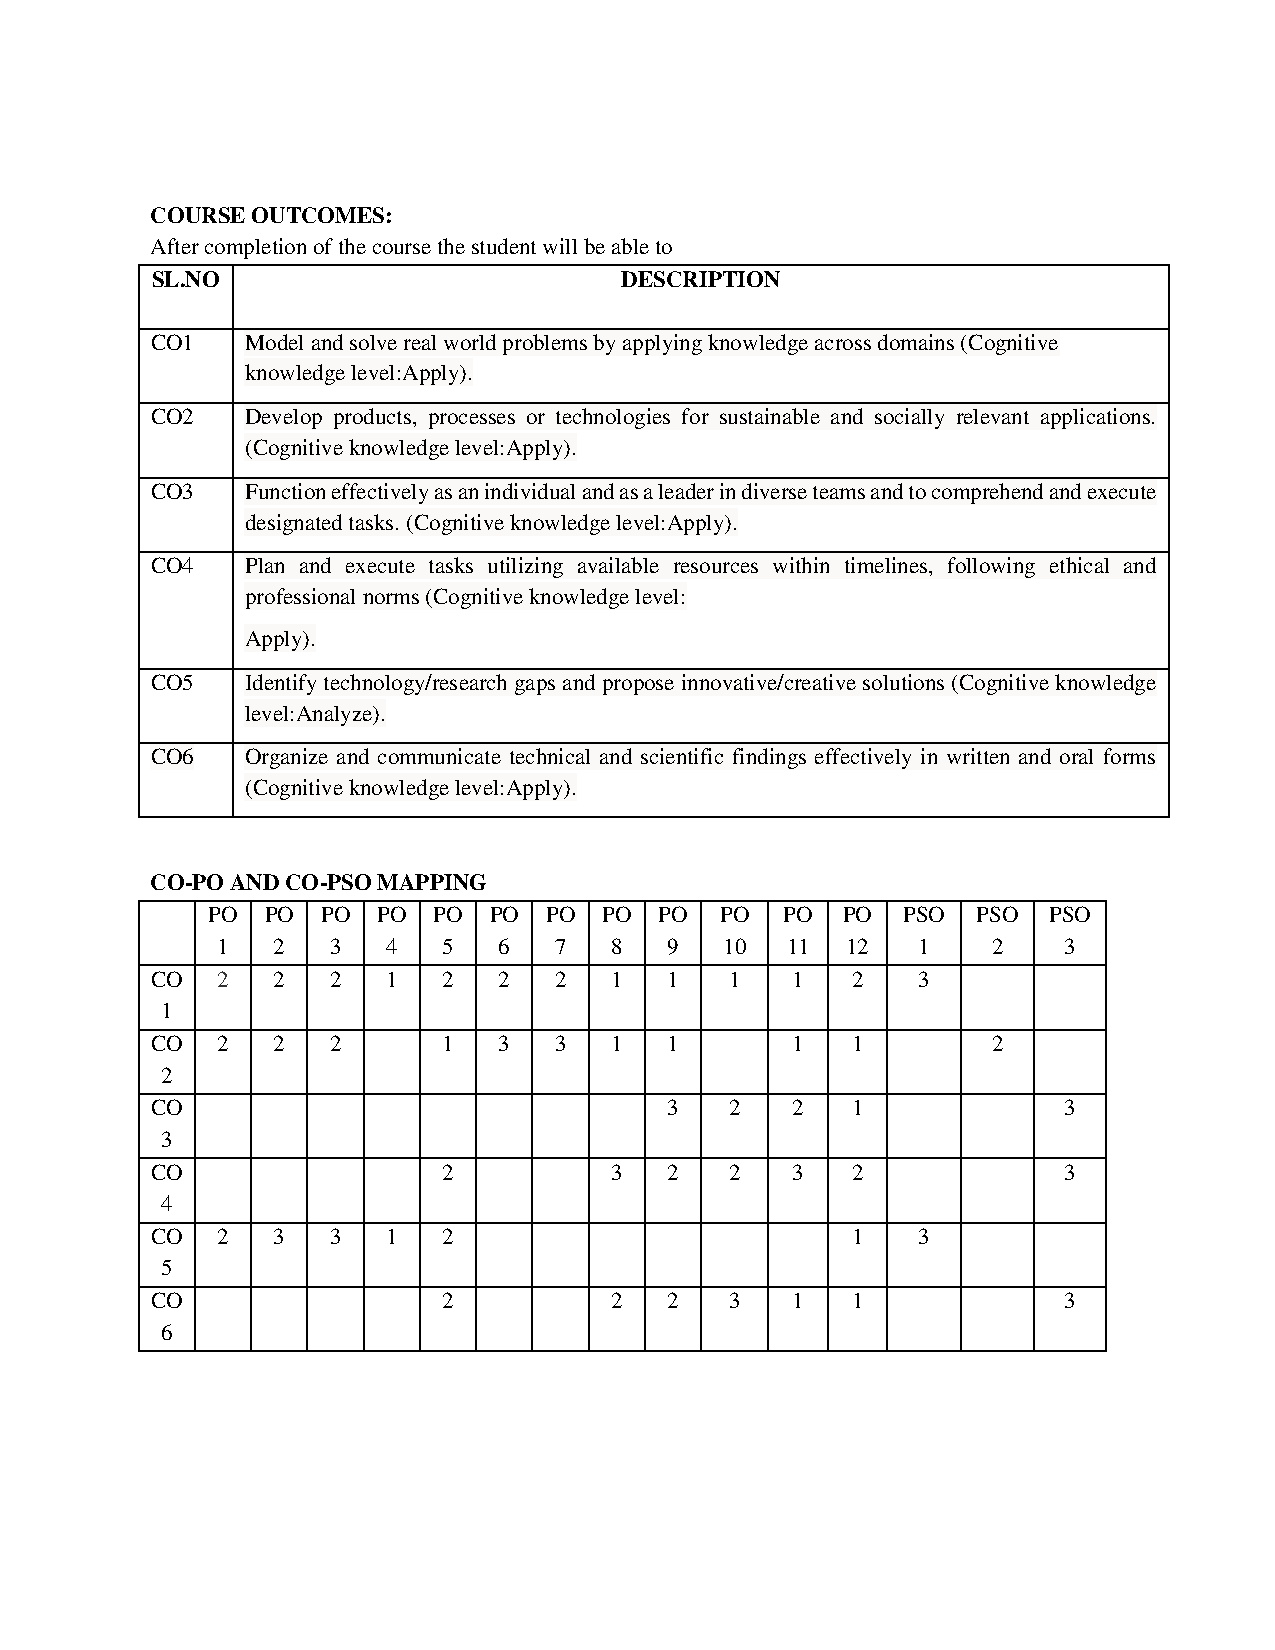
\includepdf[pages=-]{CO & jUSTIFICATIONS.pdf}
	
	\clearpage

\clearpage

% \addcontentsline{toc}{chapter}{Appendix D: CO-PO-PSO Mapping}
% \chapter*{}
% \paragraph\
% \vspace{75mm}
% \begin{center}
%     \textbf{\huge{Appendix D: }}
%     \textbf{\huge{CO-PO-PSO Mapping}}
% \end{center}
% \clearpage
% \clearpage





\vspace{1cm}

\begin{table}[htp]
\centering
\caption*{CO-PO AND CO-PSO MAPPING}
\scalebox{0.75}{
\begin{tabular}{|p{0.8cm}|p{0.8cm}|p{0.8cm}|p{0.8cm}|p{0.8cm}|p{0.8cm}|p{0.8cm}|p{0.8cm}|p{0.8cm}|p{0.8cm}|p{0.8cm}|p{0.8cm}|p{0.8cm}|p{0.8cm}|p{0.8cm}|p{0.8cm}|}
\hline
\textbf{} & \textbf{PO
1} & \textbf{PO
2} & \textbf{PO
3} & \textbf{PO
4} & \textbf{PO
5} & \textbf{PO
6} & \textbf{PO
7} & \textbf{PO
8} & \textbf{PO
9} & \textbf{PO
10} & \textbf{PO
11} & \textbf{PO
12} & \textbf{PSO
1} & \textbf{PSO
2} & \textbf{PSO
3} \\
\hline
\textbf{CO
1} & 2 & 2 & 2 & 1 & 2 & 2 & 2 & 1 & 1 & 1 & 1 & 2 & 3 & & \\ \hline
\textbf{CO
2} & 2 & 2 & 2 & & 1 & 3 & 3 & 1 & 1 & & 1 & 1 & & 2 & \\ \hline
\textbf{CO
3} & & & & & & & & & 3 & 2 & 2 & 1 & & & 3 \\ \hline
\textbf{CO
4} & & & & & 2 & & & 3 & 2 & 2 & 3 & 2 & & & 3 \\ \hline
\textbf{CO
5} & 2 & 3 & 3 & 1 & 2 & & & & & & & 1 & 3 & & \\ \hline
\textbf{CO
6} & & & & & 2 & & & 2 & 2 & 3 & 1 & 1 & & & 3 \\
\hline
\end{tabular}}
\end{table}



\clearpage
\thispagestyle{plain}
\begin{center}
    \large{\textbf{JUSTIFICATIONS FOR CO-PO MAPPING}}
\end{center}

\begin{longtable}{|p{4.5cm}|p{1.5cm}|p{8.5cm}|}
\hline
\textbf{Mapping ID} & \textbf{Level} & \textbf{Justification} \\
\hline
\endfirsthead
% \multicolumn{3}{c}{\tablename\ \thetable\ -- Continued} \\
\hline
\textbf{Mapping ID} & \textbf{Level} & \textbf{Justification} \\
\hline
\endhead
\hline
\endfoot
\hline
\endlastfoot

101003/ CS722U.1-PO1 & M & Knowledge in the area of technology for project development using various tools results in better modeling. \\ \hline
101003/ CS722U.1-PO2 & M & Knowledge acquired in the selected area of project development can be used to identify, formulate, review research literature, and analyze complex engineering problems reaching substantiated conclusions. \\ \hline
101003/ CS722U.1-PO3 & M & Can use the acquired knowledge in designing solutions to complex problems. \\ \hline
101003/ CS722U.1-PO4 & M & Can use the acquired knowledge in designing solutions to complex problems. \\ \hline
101003/ CS722U.1-PO5 & H & Students are able to interpret, improve and redefine technical aspects for design of experiments, analysis and interpretation of data, and synthesis of the information to provide valid conclusions. \\ \hline
101003/ CS722U.1-PO6 & M & Students are able to interpret, improve and redefine technical aspects by applying contextual knowledge to assess societal, health and consequential responsibilities relevant to professional engineering practices. \\ \hline
101003/ CS722U.1-PO7 & M & Project development based on societal and environmental context solution identification is the need for sustainable development. \\ \hline
101003/ CS722U.1-PO8 & L & Project development should be based on professional ethics and responsibilities. \\ \hline
101003/ CS722U.1-PO9 & L & Project development using a systematic approach based on well defined principles will result in teamwork. \\ \hline
101003/ CS722U.1-PO10 & M & Project brings technological changes in society. \\ \hline
101003/ CS722U.1-PO11 & H & Acquiring knowledge for project development gathers skills in design, analysis, development and implementation of algorithms. \\ \hline
101003/ CS722U.1-PO12 & H & Knowledge for project development contributes engineering skills in computing \& information gatherings. \\ \hline

101003/ CS722U.2-PO1 & H & Knowledge acquired for project development will also include systematic planning, developing, testing and implementation in computer science solutions in various domains. \\ \hline
101003/ CS722U.2-PO2 & H & Project design and development using a systematic approach brings knowledge in mathematics and engineering fundamentals. \\ \hline
101003/ CS722U.2-PO3 & H & Identifying, formulating and analyzing the project results in a systematic approach. \\ \hline
101003/ CS722U.2-PO5 & H & Systematic approach is the tip for solving complex problems in various domains. \\ \hline
101003/ CS722U.2-PO6 & H & Systematic approach in the technical and design aspects provide valid conclusions. \\ \hline
101003/ CS722U.2-PO7 & H & Systematic approach in the technical and design aspects demonstrate the knowledge of sustainable development. \\ \hline
101003/ CS722U.2-PO8 & M & Identification and justification of technical aspects of project development demonstrates the need for sustainable development. \\ \hline
101003/ CS722U.2-PO9 & H & Apply professional ethics and responsibilities in engineering practice of development. \\ \hline
101003/ CS722U.2-PO11 & H & Systematic approach also includes effective reporting and documentation which gives clear instructions. \\ \hline
101003/ CS722U.2-PO12 & M & Project development using a systematic approach based on well defined principles will result in better teamwork. \\ \hline

101003/ CS722U.3-PO9 & H & Project development as a team brings the ability to engage in independent and lifelong learning. \\ \hline
101003/ CS722U.3-PO10 & H & Identification, formulation and justification in technical aspects will be based on acquiring skills in design and development of algorithms. \\ \hline
101003/ CS722U.3-PO11 & H & Identification, formulation and justification in technical aspects provides the betterment of life in various domains. \\ \hline
101003/ CS722U.3-PO12 & H & Students are able to interpret, improve and redefine technical aspects with mathematics, science and engineering fundamentals for the solutions of complex problems. \\ \hline

101003/ CS722U.4-PO5 & H & Students are able to interpret, improve and redefine technical aspects with identification formulation and analysis of complex problems. \\ \hline
101003/ CS722U.4-PO8 & H & Students are able to interpret, improve and redefine technical aspects to meet the specified needs with appropriate consideration for the public health and safety, and the cultural, societal, and environmental considerations. \\ \hline
101003/ CS722U.4-PO9 & H & Students are able to interpret, improve and redefine technical aspects for design of experiments, analysis and interpretation of data, and synthesis of the information to provide valid conclusions. \\ \hline
101003/ CS722U.4-PO10 & H & Create, select, and apply appropriate techniques, resources, and modern engineering and IT tools for better products. \\ \hline
101003/ CS722U.4-PO11 & M & Students are able to interpret, improve and redefine technical aspects by applying contextual knowledge to assess societal, health and consequential responsibilities relevant to professional engineering practices. \\ \hline
101003/ CS722U.4-PO12 & H & Students are able to interpret, improve and redefine technical aspects for demonstrating the knowledge of, and need for sustainable development. \\ \hline

101003/ CS722U.5-PO1 & H & Students are able to interpret, improve and redefine technical aspects, apply ethical principles and commit to professional ethics and responsibilities and norms of engineering practice. \\ \hline
101003/ CS722U.5-PO2 & M & Students are able to interpret, improve and redefine technical aspects, communicate effectively on complex engineering activities with the engineering community and with society at large, such as, being able to comprehend and write effective reports and design documentation, make effective presentations, and give and receive clear instructions. \\ \hline
101003/ CS722U.5-PO3 & H & Students are able to interpret, improve and redefine technical aspects to demonstrate knowledge and understanding of the engineering and management principles in multidisciplinary environments. \\ \hline
101003/ CS722U.5-PO4 & H & Students can interpret, improve and redefine technical aspects, recognize the need for, and have the preparation and ability to engage in independent and life-long learning in the broadest context of technological change. \\ \hline
101003/ CS722U.5-PO5 & M & Students are able to interpret, improve and redefine technical aspects in acquiring skills to design, analyze and develop algorithms and implement those using high-level programming languages. \\ \hline
101003/ CS722U.5-PO12 & M & Students are able to interpret, improve and redefine technical aspects and contribute their engineering skills in computing and information engineering domains like network design and administration, database design and knowledge engineering. \\ \hline

101003/ CS722U.6-PO5 & M & Students are able to interpret, improve and redefine technical aspects and develop strong skills in systematic planning, developing, testing, implementing and providing IT solutions for different domains which help in the betterment of life. \\ \hline
101003/ CS722U.6-PO8 & H & Students will be able to associate with a team as an effective team player for the development of technical projects by applying the knowledge of mathematics, science, engineering fundamentals, and an engineering specialization to the solution of complex engineering problems. \\ \hline
101003/ CS722U.6-PO9 & H & Students will be able to associate with a team as an effective team player for Identify, formulate, review research literature, and analyze complex engineering problems. \\ \hline
101003/ CS722U.6-PO10 & M & Students will be able to associate with a team as an effective team player for designing solutions to complex engineering problems and design system components. \\ \hline
101003/ CS722U.6-PO11 & M & Students will be able to associate with a team as an effective team player using research-based knowledge and research methods including design of experiments, analysis and interpretation of data. \\ \hline
101003/ CS722U.6-PO12 & H & Students will be able to associate with a team as an effective team player, applying ethical principles and committing to professional ethics and responsibilities and norms of engineering practice. \\ \hline
101003/ CS722U.1-PSO1 & H & Students can develop Computer Science Specific Skills by modeling and solving problems. \\ \hline
101003/ CS722U.2-PSO2 & M & Developing products, processes or technologies for sustainable and socially relevant applications can promote Programming and Software Development Skills. \\ \hline
101003/ CS722U.3-PSO3 & H & Working in a team can result in the effective development of Professional Skills. \\ \hline
101003/ CS722U.4-PSO3 & H & Planning and scheduling can result in the effective development of Professional Skills. \\ \hline
101003/ CS722U.5-PSO1 & H & Students can develop Computer Science Specific Skills by creating innovative solutions to problems. \\ \hline
101003/ CS722U.6-PSO3 & H & Organizing and communicating technical and scientific findings can help in the effective development of Professional Skills. \\ \hline
\end{longtable}

\clearpage
	\addcontentsline{toc}{chapter}{Appendix C: CO--PO--PSO Mapping}
	\chapter*{}
	\paragraph\ 
	\vspace{75mm}
	\begin{center}
		\textbf{\huge{Appendix C: }}
		\textbf{\huge{CO--PO--PSO Mapping}}
	\end{center}
	% 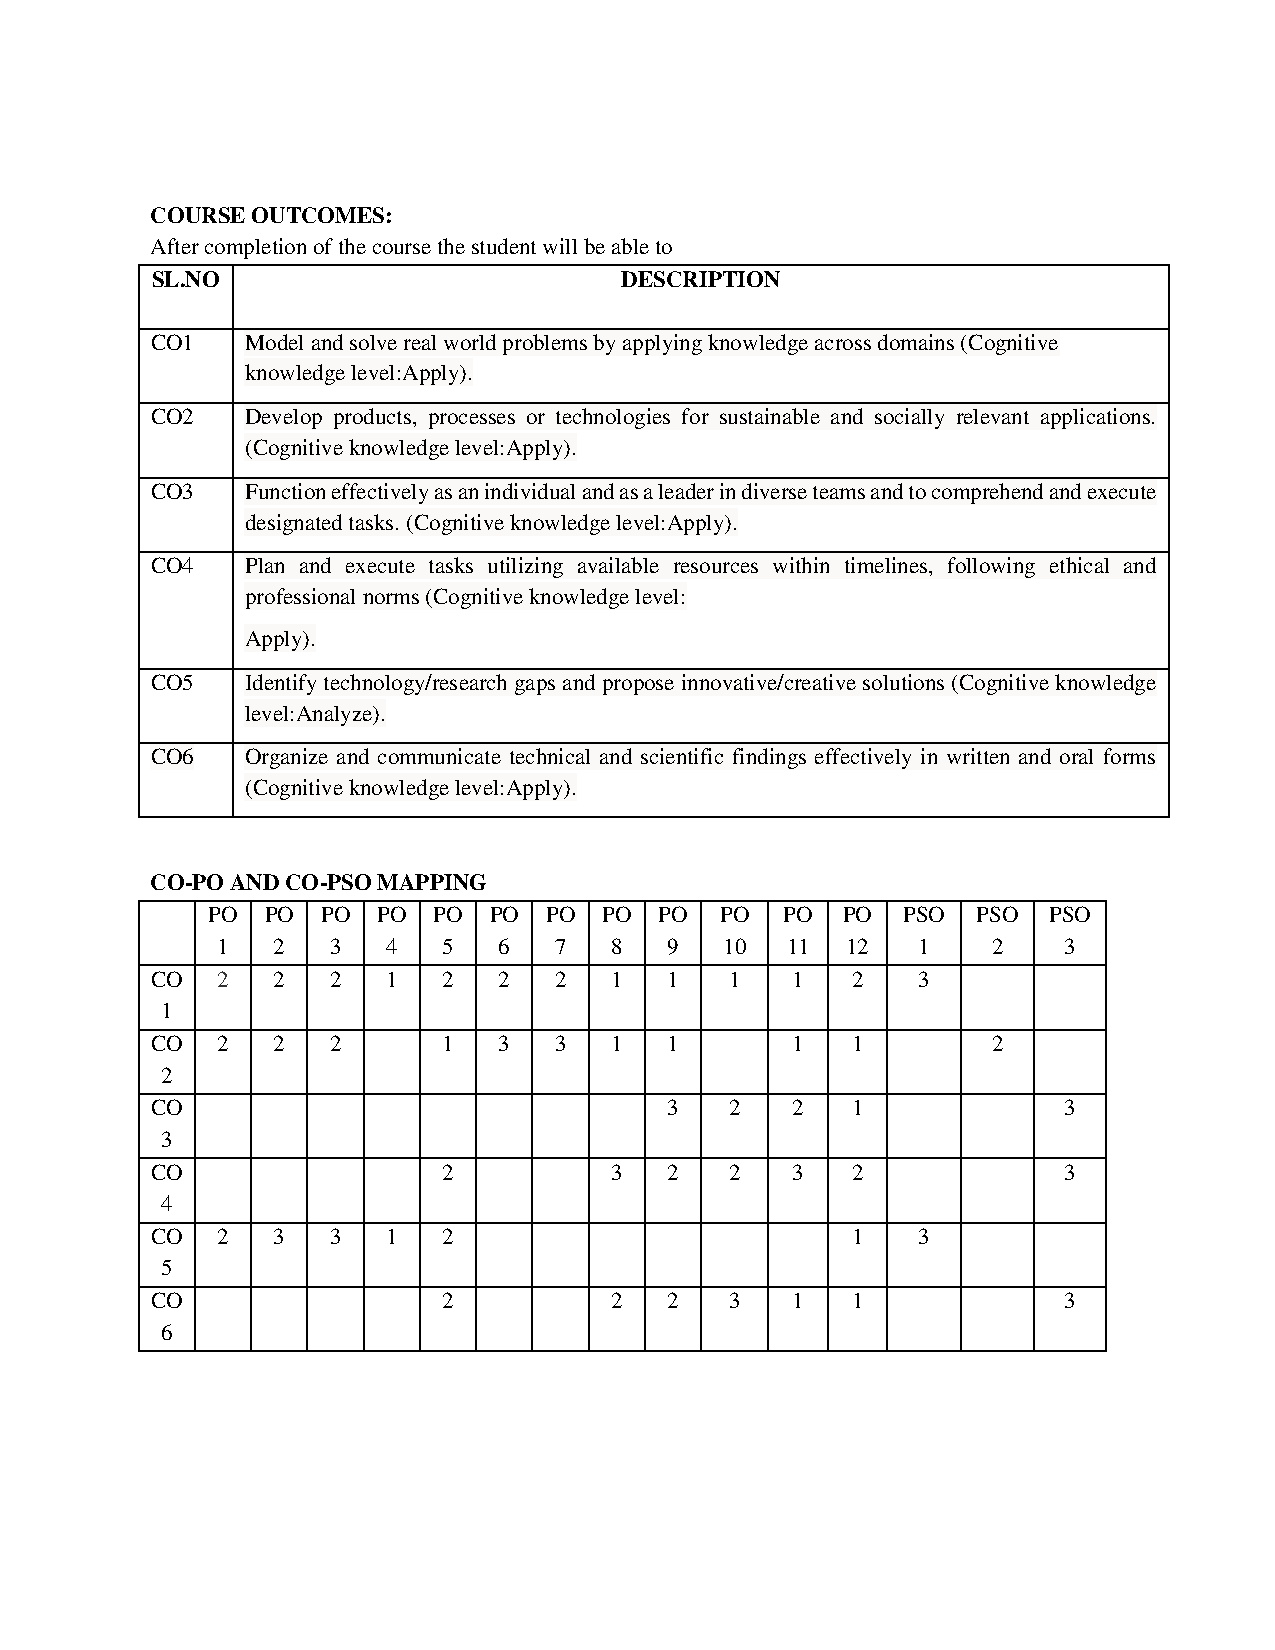
\includepdf[pages=-]{CO & jUSTIFICATIONS.pdf}
	
	\clearpage

\clearpage

% \addcontentsline{toc}{chapter}{Appendix D: CO-PO-PSO Mapping}
% \chapter*{}
% \paragraph\
% \vspace{75mm}
% \begin{center}
%     \textbf{\huge{Appendix D: }}
%     \textbf{\huge{CO-PO-PSO Mapping}}
% \end{center}
% \clearpage
% \clearpage





\vspace{1cm}

\begin{table}[htp]
\centering
\caption*{CO-PO AND CO-PSO MAPPING}
\scalebox{0.75}{
\begin{tabular}{|p{0.8cm}|p{0.8cm}|p{0.8cm}|p{0.8cm}|p{0.8cm}|p{0.8cm}|p{0.8cm}|p{0.8cm}|p{0.8cm}|p{0.8cm}|p{0.8cm}|p{0.8cm}|p{0.8cm}|p{0.8cm}|p{0.8cm}|p{0.8cm}|}
\hline
\textbf{} & \textbf{PO
1} & \textbf{PO
2} & \textbf{PO
3} & \textbf{PO
4} & \textbf{PO
5} & \textbf{PO
6} & \textbf{PO
7} & \textbf{PO
8} & \textbf{PO
9} & \textbf{PO
10} & \textbf{PO
11} & \textbf{PO
12} & \textbf{PSO
1} & \textbf{PSO
2} & \textbf{PSO
3} \\
\hline
\textbf{CO
1} & 2 & 2 & 2 & 1 & 2 & 2 & 2 & 1 & 1 & 1 & 1 & 2 & 3 & & \\ \hline
\textbf{CO
2} & 2 & 2 & 2 & & 1 & 3 & 3 & 1 & 1 & & 1 & 1 & & 2 & \\ \hline
\textbf{CO
3} & & & & & & & & & 3 & 2 & 2 & 1 & & & 3 \\ \hline
\textbf{CO
4} & & & & & 2 & & & 3 & 2 & 2 & 3 & 2 & & & 3 \\ \hline
\textbf{CO
5} & 2 & 3 & 3 & 1 & 2 & & & & & & & 1 & 3 & & \\ \hline
\textbf{CO
6} & & & & & 2 & & & 2 & 2 & 3 & 1 & 1 & & & 3 \\
\hline
\end{tabular}}
\end{table}



\clearpage
\thispagestyle{plain}
\begin{center}
    \large{\textbf{JUSTIFICATIONS FOR CO-PO MAPPING}}
\end{center}

\begin{longtable}{|p{4.5cm}|p{1.5cm}|p{8.5cm}|}
\hline
\textbf{Mapping ID} & \textbf{Level} & \textbf{Justification} \\
\hline
\endfirsthead
% \multicolumn{3}{c}{\tablename\ \thetable\ -- Continued} \\
\hline
\textbf{Mapping ID} & \textbf{Level} & \textbf{Justification} \\
\hline
\endhead
\hline
\endfoot
\hline
\endlastfoot

101003/ CS722U.1-PO1 & M & Knowledge in the area of technology for project development using various tools results in better modeling. \\ \hline
101003/ CS722U.1-PO2 & M & Knowledge acquired in the selected area of project development can be used to identify, formulate, review research literature, and analyze complex engineering problems reaching substantiated conclusions. \\ \hline
101003/ CS722U.1-PO3 & M & Can use the acquired knowledge in designing solutions to complex problems. \\ \hline
101003/ CS722U.1-PO4 & M & Can use the acquired knowledge in designing solutions to complex problems. \\ \hline
101003/ CS722U.1-PO5 & H & Students are able to interpret, improve and redefine technical aspects for design of experiments, analysis and interpretation of data, and synthesis of the information to provide valid conclusions. \\ \hline
101003/ CS722U.1-PO6 & M & Students are able to interpret, improve and redefine technical aspects by applying contextual knowledge to assess societal, health and consequential responsibilities relevant to professional engineering practices. \\ \hline
101003/ CS722U.1-PO7 & M & Project development based on societal and environmental context solution identification is the need for sustainable development. \\ \hline
101003/ CS722U.1-PO8 & L & Project development should be based on professional ethics and responsibilities. \\ \hline
101003/ CS722U.1-PO9 & L & Project development using a systematic approach based on well defined principles will result in teamwork. \\ \hline
101003/ CS722U.1-PO10 & M & Project brings technological changes in society. \\ \hline
101003/ CS722U.1-PO11 & H & Acquiring knowledge for project development gathers skills in design, analysis, development and implementation of algorithms. \\ \hline
101003/ CS722U.1-PO12 & H & Knowledge for project development contributes engineering skills in computing \& information gatherings. \\ \hline

101003/ CS722U.2-PO1 & H & Knowledge acquired for project development will also include systematic planning, developing, testing and implementation in computer science solutions in various domains. \\ \hline
101003/ CS722U.2-PO2 & H & Project design and development using a systematic approach brings knowledge in mathematics and engineering fundamentals. \\ \hline
101003/ CS722U.2-PO3 & H & Identifying, formulating and analyzing the project results in a systematic approach. \\ \hline
101003/ CS722U.2-PO5 & H & Systematic approach is the tip for solving complex problems in various domains. \\ \hline
101003/ CS722U.2-PO6 & H & Systematic approach in the technical and design aspects provide valid conclusions. \\ \hline
101003/ CS722U.2-PO7 & H & Systematic approach in the technical and design aspects demonstrate the knowledge of sustainable development. \\ \hline
101003/ CS722U.2-PO8 & M & Identification and justification of technical aspects of project development demonstrates the need for sustainable development. \\ \hline
101003/ CS722U.2-PO9 & H & Apply professional ethics and responsibilities in engineering practice of development. \\ \hline
101003/ CS722U.2-PO11 & H & Systematic approach also includes effective reporting and documentation which gives clear instructions. \\ \hline
101003/ CS722U.2-PO12 & M & Project development using a systematic approach based on well defined principles will result in better teamwork. \\ \hline

101003/ CS722U.3-PO9 & H & Project development as a team brings the ability to engage in independent and lifelong learning. \\ \hline
101003/ CS722U.3-PO10 & H & Identification, formulation and justification in technical aspects will be based on acquiring skills in design and development of algorithms. \\ \hline
101003/ CS722U.3-PO11 & H & Identification, formulation and justification in technical aspects provides the betterment of life in various domains. \\ \hline
101003/ CS722U.3-PO12 & H & Students are able to interpret, improve and redefine technical aspects with mathematics, science and engineering fundamentals for the solutions of complex problems. \\ \hline

101003/ CS722U.4-PO5 & H & Students are able to interpret, improve and redefine technical aspects with identification formulation and analysis of complex problems. \\ \hline
101003/ CS722U.4-PO8 & H & Students are able to interpret, improve and redefine technical aspects to meet the specified needs with appropriate consideration for the public health and safety, and the cultural, societal, and environmental considerations. \\ \hline
101003/ CS722U.4-PO9 & H & Students are able to interpret, improve and redefine technical aspects for design of experiments, analysis and interpretation of data, and synthesis of the information to provide valid conclusions. \\ \hline
101003/ CS722U.4-PO10 & H & Create, select, and apply appropriate techniques, resources, and modern engineering and IT tools for better products. \\ \hline
101003/ CS722U.4-PO11 & M & Students are able to interpret, improve and redefine technical aspects by applying contextual knowledge to assess societal, health and consequential responsibilities relevant to professional engineering practices. \\ \hline
101003/ CS722U.4-PO12 & H & Students are able to interpret, improve and redefine technical aspects for demonstrating the knowledge of, and need for sustainable development. \\ \hline

101003/ CS722U.5-PO1 & H & Students are able to interpret, improve and redefine technical aspects, apply ethical principles and commit to professional ethics and responsibilities and norms of engineering practice. \\ \hline
101003/ CS722U.5-PO2 & M & Students are able to interpret, improve and redefine technical aspects, communicate effectively on complex engineering activities with the engineering community and with society at large, such as, being able to comprehend and write effective reports and design documentation, make effective presentations, and give and receive clear instructions. \\ \hline
101003/ CS722U.5-PO3 & H & Students are able to interpret, improve and redefine technical aspects to demonstrate knowledge and understanding of the engineering and management principles in multidisciplinary environments. \\ \hline
101003/ CS722U.5-PO4 & H & Students can interpret, improve and redefine technical aspects, recognize the need for, and have the preparation and ability to engage in independent and life-long learning in the broadest context of technological change. \\ \hline
101003/ CS722U.5-PO5 & M & Students are able to interpret, improve and redefine technical aspects in acquiring skills to design, analyze and develop algorithms and implement those using high-level programming languages. \\ \hline
101003/ CS722U.5-PO12 & M & Students are able to interpret, improve and redefine technical aspects and contribute their engineering skills in computing and information engineering domains like network design and administration, database design and knowledge engineering. \\ \hline

101003/ CS722U.6-PO5 & M & Students are able to interpret, improve and redefine technical aspects and develop strong skills in systematic planning, developing, testing, implementing and providing IT solutions for different domains which help in the betterment of life. \\ \hline
101003/ CS722U.6-PO8 & H & Students will be able to associate with a team as an effective team player for the development of technical projects by applying the knowledge of mathematics, science, engineering fundamentals, and an engineering specialization to the solution of complex engineering problems. \\ \hline
101003/ CS722U.6-PO9 & H & Students will be able to associate with a team as an effective team player for Identify, formulate, review research literature, and analyze complex engineering problems. \\ \hline
101003/ CS722U.6-PO10 & M & Students will be able to associate with a team as an effective team player for designing solutions to complex engineering problems and design system components. \\ \hline
101003/ CS722U.6-PO11 & M & Students will be able to associate with a team as an effective team player using research-based knowledge and research methods including design of experiments, analysis and interpretation of data. \\ \hline
101003/ CS722U.6-PO12 & H & Students will be able to associate with a team as an effective team player, applying ethical principles and committing to professional ethics and responsibilities and norms of engineering practice. \\ \hline
101003/ CS722U.1-PSO1 & H & Students can develop Computer Science Specific Skills by modeling and solving problems. \\ \hline
101003/ CS722U.2-PSO2 & M & Developing products, processes or technologies for sustainable and socially relevant applications can promote Programming and Software Development Skills. \\ \hline
101003/ CS722U.3-PSO3 & H & Working in a team can result in the effective development of Professional Skills. \\ \hline
101003/ CS722U.4-PSO3 & H & Planning and scheduling can result in the effective development of Professional Skills. \\ \hline
101003/ CS722U.5-PSO1 & H & Students can develop Computer Science Specific Skills by creating innovative solutions to problems. \\ \hline
101003/ CS722U.6-PSO3 & H & Organizing and communicating technical and scientific findings can help in the effective development of Professional Skills. \\ \hline
\end{longtable}

\clearpage
	\addcontentsline{toc}{chapter}{Appendix C: CO--PO--PSO Mapping}
	\chapter*{}
	\paragraph\ 
	\vspace{75mm}
	\begin{center}
		\textbf{\huge{Appendix C: }}
		\textbf{\huge{CO--PO--PSO Mapping}}
	\end{center}
	% 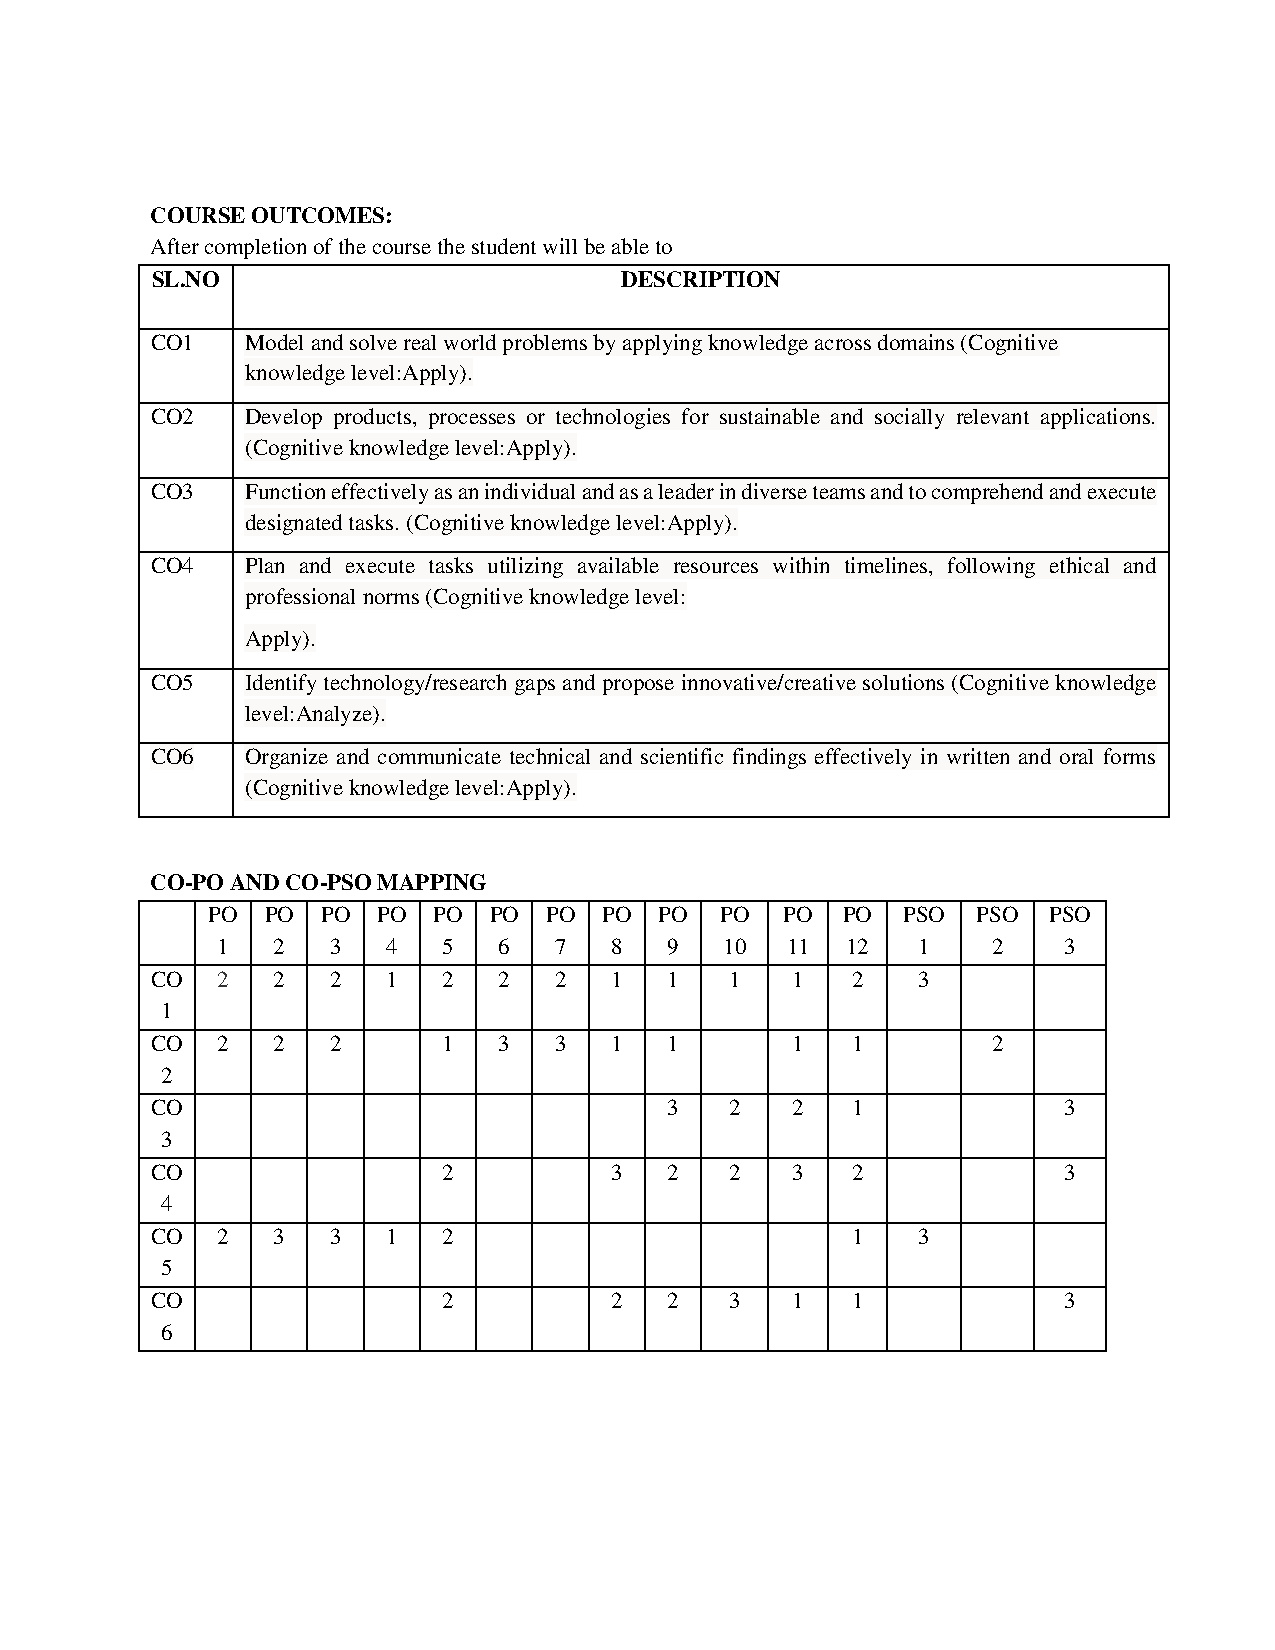
\includepdf[pages=-]{CO & jUSTIFICATIONS.pdf}
	
	\clearpage

\clearpage

% \addcontentsline{toc}{chapter}{Appendix D: CO-PO-PSO Mapping}
% \chapter*{}
% \paragraph\
% \vspace{75mm}
% \begin{center}
%     \textbf{\huge{Appendix D: }}
%     \textbf{\huge{CO-PO-PSO Mapping}}
% \end{center}
% \clearpage
% \clearpage





\vspace{1cm}

\begin{table}[htp]
\centering
\caption*{CO-PO AND CO-PSO MAPPING}
\scalebox{0.75}{
\begin{tabular}{|p{0.8cm}|p{0.8cm}|p{0.8cm}|p{0.8cm}|p{0.8cm}|p{0.8cm}|p{0.8cm}|p{0.8cm}|p{0.8cm}|p{0.8cm}|p{0.8cm}|p{0.8cm}|p{0.8cm}|p{0.8cm}|p{0.8cm}|p{0.8cm}|}
\hline
\textbf{} & \textbf{PO
1} & \textbf{PO
2} & \textbf{PO
3} & \textbf{PO
4} & \textbf{PO
5} & \textbf{PO
6} & \textbf{PO
7} & \textbf{PO
8} & \textbf{PO
9} & \textbf{PO
10} & \textbf{PO
11} & \textbf{PO
12} & \textbf{PSO
1} & \textbf{PSO
2} & \textbf{PSO
3} \\
\hline
\textbf{CO
1} & 2 & 2 & 2 & 1 & 2 & 2 & 2 & 1 & 1 & 1 & 1 & 2 & 3 & & \\ \hline
\textbf{CO
2} & 2 & 2 & 2 & & 1 & 3 & 3 & 1 & 1 & & 1 & 1 & & 2 & \\ \hline
\textbf{CO
3} & & & & & & & & & 3 & 2 & 2 & 1 & & & 3 \\ \hline
\textbf{CO
4} & & & & & 2 & & & 3 & 2 & 2 & 3 & 2 & & & 3 \\ \hline
\textbf{CO
5} & 2 & 3 & 3 & 1 & 2 & & & & & & & 1 & 3 & & \\ \hline
\textbf{CO
6} & & & & & 2 & & & 2 & 2 & 3 & 1 & 1 & & & 3 \\
\hline
\end{tabular}}
\end{table}



\clearpage
\thispagestyle{plain}
\begin{center}
    \large{\textbf{JUSTIFICATIONS FOR CO-PO MAPPING}}
\end{center}

\begin{longtable}{|p{4.5cm}|p{1.5cm}|p{8.5cm}|}
\hline
\textbf{Mapping ID} & \textbf{Level} & \textbf{Justification} \\
\hline
\endfirsthead
% \multicolumn{3}{c}{\tablename\ \thetable\ -- Continued} \\
\hline
\textbf{Mapping ID} & \textbf{Level} & \textbf{Justification} \\
\hline
\endhead
\hline
\endfoot
\hline
\endlastfoot

101003/ CS722U.1-PO1 & M & Knowledge in the area of technology for project development using various tools results in better modeling. \\ \hline
101003/ CS722U.1-PO2 & M & Knowledge acquired in the selected area of project development can be used to identify, formulate, review research literature, and analyze complex engineering problems reaching substantiated conclusions. \\ \hline
101003/ CS722U.1-PO3 & M & Can use the acquired knowledge in designing solutions to complex problems. \\ \hline
101003/ CS722U.1-PO4 & M & Can use the acquired knowledge in designing solutions to complex problems. \\ \hline
101003/ CS722U.1-PO5 & H & Students are able to interpret, improve and redefine technical aspects for design of experiments, analysis and interpretation of data, and synthesis of the information to provide valid conclusions. \\ \hline
101003/ CS722U.1-PO6 & M & Students are able to interpret, improve and redefine technical aspects by applying contextual knowledge to assess societal, health and consequential responsibilities relevant to professional engineering practices. \\ \hline
101003/ CS722U.1-PO7 & M & Project development based on societal and environmental context solution identification is the need for sustainable development. \\ \hline
101003/ CS722U.1-PO8 & L & Project development should be based on professional ethics and responsibilities. \\ \hline
101003/ CS722U.1-PO9 & L & Project development using a systematic approach based on well defined principles will result in teamwork. \\ \hline
101003/ CS722U.1-PO10 & M & Project brings technological changes in society. \\ \hline
101003/ CS722U.1-PO11 & H & Acquiring knowledge for project development gathers skills in design, analysis, development and implementation of algorithms. \\ \hline
101003/ CS722U.1-PO12 & H & Knowledge for project development contributes engineering skills in computing \& information gatherings. \\ \hline

101003/ CS722U.2-PO1 & H & Knowledge acquired for project development will also include systematic planning, developing, testing and implementation in computer science solutions in various domains. \\ \hline
101003/ CS722U.2-PO2 & H & Project design and development using a systematic approach brings knowledge in mathematics and engineering fundamentals. \\ \hline
101003/ CS722U.2-PO3 & H & Identifying, formulating and analyzing the project results in a systematic approach. \\ \hline
101003/ CS722U.2-PO5 & H & Systematic approach is the tip for solving complex problems in various domains. \\ \hline
101003/ CS722U.2-PO6 & H & Systematic approach in the technical and design aspects provide valid conclusions. \\ \hline
101003/ CS722U.2-PO7 & H & Systematic approach in the technical and design aspects demonstrate the knowledge of sustainable development. \\ \hline
101003/ CS722U.2-PO8 & M & Identification and justification of technical aspects of project development demonstrates the need for sustainable development. \\ \hline
101003/ CS722U.2-PO9 & H & Apply professional ethics and responsibilities in engineering practice of development. \\ \hline
101003/ CS722U.2-PO11 & H & Systematic approach also includes effective reporting and documentation which gives clear instructions. \\ \hline
101003/ CS722U.2-PO12 & M & Project development using a systematic approach based on well defined principles will result in better teamwork. \\ \hline

101003/ CS722U.3-PO9 & H & Project development as a team brings the ability to engage in independent and lifelong learning. \\ \hline
101003/ CS722U.3-PO10 & H & Identification, formulation and justification in technical aspects will be based on acquiring skills in design and development of algorithms. \\ \hline
101003/ CS722U.3-PO11 & H & Identification, formulation and justification in technical aspects provides the betterment of life in various domains. \\ \hline
101003/ CS722U.3-PO12 & H & Students are able to interpret, improve and redefine technical aspects with mathematics, science and engineering fundamentals for the solutions of complex problems. \\ \hline

101003/ CS722U.4-PO5 & H & Students are able to interpret, improve and redefine technical aspects with identification formulation and analysis of complex problems. \\ \hline
101003/ CS722U.4-PO8 & H & Students are able to interpret, improve and redefine technical aspects to meet the specified needs with appropriate consideration for the public health and safety, and the cultural, societal, and environmental considerations. \\ \hline
101003/ CS722U.4-PO9 & H & Students are able to interpret, improve and redefine technical aspects for design of experiments, analysis and interpretation of data, and synthesis of the information to provide valid conclusions. \\ \hline
101003/ CS722U.4-PO10 & H & Create, select, and apply appropriate techniques, resources, and modern engineering and IT tools for better products. \\ \hline
101003/ CS722U.4-PO11 & M & Students are able to interpret, improve and redefine technical aspects by applying contextual knowledge to assess societal, health and consequential responsibilities relevant to professional engineering practices. \\ \hline
101003/ CS722U.4-PO12 & H & Students are able to interpret, improve and redefine technical aspects for demonstrating the knowledge of, and need for sustainable development. \\ \hline

101003/ CS722U.5-PO1 & H & Students are able to interpret, improve and redefine technical aspects, apply ethical principles and commit to professional ethics and responsibilities and norms of engineering practice. \\ \hline
101003/ CS722U.5-PO2 & M & Students are able to interpret, improve and redefine technical aspects, communicate effectively on complex engineering activities with the engineering community and with society at large, such as, being able to comprehend and write effective reports and design documentation, make effective presentations, and give and receive clear instructions. \\ \hline
101003/ CS722U.5-PO3 & H & Students are able to interpret, improve and redefine technical aspects to demonstrate knowledge and understanding of the engineering and management principles in multidisciplinary environments. \\ \hline
101003/ CS722U.5-PO4 & H & Students can interpret, improve and redefine technical aspects, recognize the need for, and have the preparation and ability to engage in independent and life-long learning in the broadest context of technological change. \\ \hline
101003/ CS722U.5-PO5 & M & Students are able to interpret, improve and redefine technical aspects in acquiring skills to design, analyze and develop algorithms and implement those using high-level programming languages. \\ \hline
101003/ CS722U.5-PO12 & M & Students are able to interpret, improve and redefine technical aspects and contribute their engineering skills in computing and information engineering domains like network design and administration, database design and knowledge engineering. \\ \hline

101003/ CS722U.6-PO5 & M & Students are able to interpret, improve and redefine technical aspects and develop strong skills in systematic planning, developing, testing, implementing and providing IT solutions for different domains which help in the betterment of life. \\ \hline
101003/ CS722U.6-PO8 & H & Students will be able to associate with a team as an effective team player for the development of technical projects by applying the knowledge of mathematics, science, engineering fundamentals, and an engineering specialization to the solution of complex engineering problems. \\ \hline
101003/ CS722U.6-PO9 & H & Students will be able to associate with a team as an effective team player for Identify, formulate, review research literature, and analyze complex engineering problems. \\ \hline
101003/ CS722U.6-PO10 & M & Students will be able to associate with a team as an effective team player for designing solutions to complex engineering problems and design system components. \\ \hline
101003/ CS722U.6-PO11 & M & Students will be able to associate with a team as an effective team player using research-based knowledge and research methods including design of experiments, analysis and interpretation of data. \\ \hline
101003/ CS722U.6-PO12 & H & Students will be able to associate with a team as an effective team player, applying ethical principles and committing to professional ethics and responsibilities and norms of engineering practice. \\ \hline
101003/ CS722U.1-PSO1 & H & Students can develop Computer Science Specific Skills by modeling and solving problems. \\ \hline
101003/ CS722U.2-PSO2 & M & Developing products, processes or technologies for sustainable and socially relevant applications can promote Programming and Software Development Skills. \\ \hline
101003/ CS722U.3-PSO3 & H & Working in a team can result in the effective development of Professional Skills. \\ \hline
101003/ CS722U.4-PSO3 & H & Planning and scheduling can result in the effective development of Professional Skills. \\ \hline
101003/ CS722U.5-PSO1 & H & Students can develop Computer Science Specific Skills by creating innovative solutions to problems. \\ \hline
101003/ CS722U.6-PSO3 & H & Organizing and communicating technical and scientific findings can help in the effective development of Professional Skills. \\ \hline
\end{longtable}